%%%%%%%%%%%%%%%%%%%%%%%%%%%%%%%%%%%%%%%%%
% Beamer Presentation
% LaTeX Template
% Version 1.0 (10/11/12)
%
% This template has been downloaded from:
% http://www.LaTeXTemplates.com
%
% License:
% CC BY-NC-SA 3.0 (http://creativecommons.org/licenses/by-nc-sa/3.0/)
%
%%%%%%%%%%%%%%%%%%%%%%%%%%%%%%%%%%%%%%%%%

%----------------------------------------------------------------------------------------
%	PACKAGES AND THEMES
%----------------------------------------------------------------------------------------

\documentclass{beamer}

\mode<presentation> {
	
	% The Beamer class comes with a number of default slide themes
	% which change the colors and layouts of slides. Below this is a list
	% of all the themes, uncomment each in turn to see what they look like.
	
	%\usetheme{default}
	%\usetheme{AnnArbor}
	%\usetheme{Antibes}
	%\usetheme{Bergen}
	%\usetheme{Berkeley}
	%\usetheme{Berlin}
	%\usetheme{Boadilla}
	%\usetheme{CambridgeUS}
	%\usetheme{Copenhagen}
	%\usetheme{Darmstadt}
	%\usetheme{Dresden}
	%\usetheme{Frankfurt}
	%\usetheme{Goettingen}
	%\usetheme{Hannover}
	%\usetheme{Ilmenau}
	%\usetheme{JuanLesPins}
	%\usetheme{Luebeck}
	\usetheme{Madrid}
	%\usetheme{Malmoe}
	%\usetheme{Marburg}
	%\usetheme{Montpellier}
	%\usetheme{PaloAlto}
	%\usetheme{Pittsburgh}
	%\usetheme{Rochester}
	%\usetheme{Singapore}
	%\usetheme{Szeged}
	%\usetheme{Warsaw}
	
	% As well as themes, the Beamer class has a number of color themes
	% for any slide theme. Uncomment each of these in turn to see how it
	% changes the colors of your current slide theme.
	
	%\usecolortheme{albatross}
	%\usecolortheme{beaver}
	%\usecolortheme{beetle}
	%\usecolortheme{crane}
	%\usecolortheme{dolphin}
	%\usecolortheme{dove}
	%\usecolortheme{fly}
	%\usecolortheme{lily}
	%\usecolortheme{orchid}
	%\usecolortheme{rose}
	%\usecolortheme{seagull}
	%\usecolortheme{seahorse}
	%\usecolortheme{whale}
	%\usecolortheme{wolverine}
	
	%\setbeamertemplate{footline} % To remove the footer line in all slides uncomment this line
	%\setbeamertemplate{footline}[page number] % To replace the footer line in all slides with a simple slide count uncomment this line
	
	%\setbeamertemplate{navigation symbols}{} % To remove the navigation symbols from the bottom of all slides uncomment this line
}

\usepackage{amsmath}
\usepackage{graphicx} % Allows including images
\usepackage[utf8]{vietnam}
\usepackage{booktabs} % Allows the use of \toprule, \midrule and \bottomrule in tables
\usepackage[ruled,vlined]{algorithm2e}
\usepackage{algorithmic}

%----------------------------------------------------------------------------------------
%	TITLE PAGE
%----------------------------------------------------------------------------------------

\title[Project 5]{Project 5 \\
	Taxi vận chuyển người kết hợp hàng hóa} % The short title appears at the bottom of every slide, the full title is only on the title page

\author{Trần Huy Hùng\and Đỗ Ngọc Sơn} % Your name
\institute[HUST] % Your institution as it will appear on the bottom of every slide, may be shorthand to save space
{
	Đại học Bách Khoa Hà Nội \\ % Your institution for the title page
	\medskip
	% 	\textit{john@smith.com} % YourHUST email address
}
\date{\today} % Date, can be changed to a custom date

\AtBeginSection[]
{
	\begin{frame}
	\frametitle{Nội dung}
	\tableofcontents[currentsection, hideothersubsections]
	\end{frame}
}

\begin{document}
	
	\maketitle
	
	\begin{frame}
		\frametitle{Nội dung} % Table of contents slide, comment this block out to remove it
		\tableofcontents[hidesubsections]
	\end{frame}
	
	%----------------------------------------------------------------------------------------
	%	PRESENTATION SLIDES
	%----------------------------------------------------------------------------------------
	
	%------------------------------------------------
	\section{Giới thiệu bài toán} % Sections can be created in order to organize your presentation into discrete blocks, all sections and subsections are automatically printed in the table of contents as an overview of the talk
	%------------------------------------------------
	
	%\subsection{Subsection Example} % A subsection can be created just before a set of slides with a common theme to further break down your presentation into chunks
	
	\begin{frame}
		\frametitle{Giới thiệu bài toán}
		Bài toán taxi vận chuyển người kết hợp hàng hóa:
		\begin{itemize}
			\item {
				Có $N$ hành khách $(1,2,...,N)$ và $M$ gói hàng $(N+1,N+2,...,N+M)$:
				\begin{itemize}
					\item Hành khách (hoặc gói hàng) $i$ có điểm đón $i$ và điểm trả $i+N+M$ ($u=1,2,...,N+M$).
					\item Gói hàng $i$ có khối lượng $q_i$ ($i=N+1,...,N+M$).
				\end{itemize}
			}
			\item {
				Có $K$ xe taxi $(1,2,...,K)$:
				\begin{itemize}
					\item Các taxi cùng xuất phát từ điểm $0$, thực hiện các yêu cầu chở khách và hàng, rồi quay về điểm $0$.
					\item Xe taxi $k$ có thể vận chuyển cùng lúc $1$ hành khách và tối đa $Q_k$ khối lượng hàng ($k=1,2,...,K$).
					\item Taxi đã đón hành khách thì phải đi đến điểm trả khách đó ngay lập tức.
				\end{itemize}
			}
			\item $d_{ij}$ là khoảng cách từ điểm $i$ đến điểm $j$ ($i,j=0,...,2N+2M$).
		\end{itemize}
		\textbf{\underline{Yêu cầu:}} Tính toán phương án vận chuyển sao cho quãng đường di chuyển \underline{dài nhất} của các xe là \underline{ngắn nhất}.
	\end{frame}

	\begin{frame}
		\frametitle{Giới thiệu bài toán}
		\begin{figure}
			\centering
			\caption{Lộ trình đón trả người kết hợp hàng hóa}
			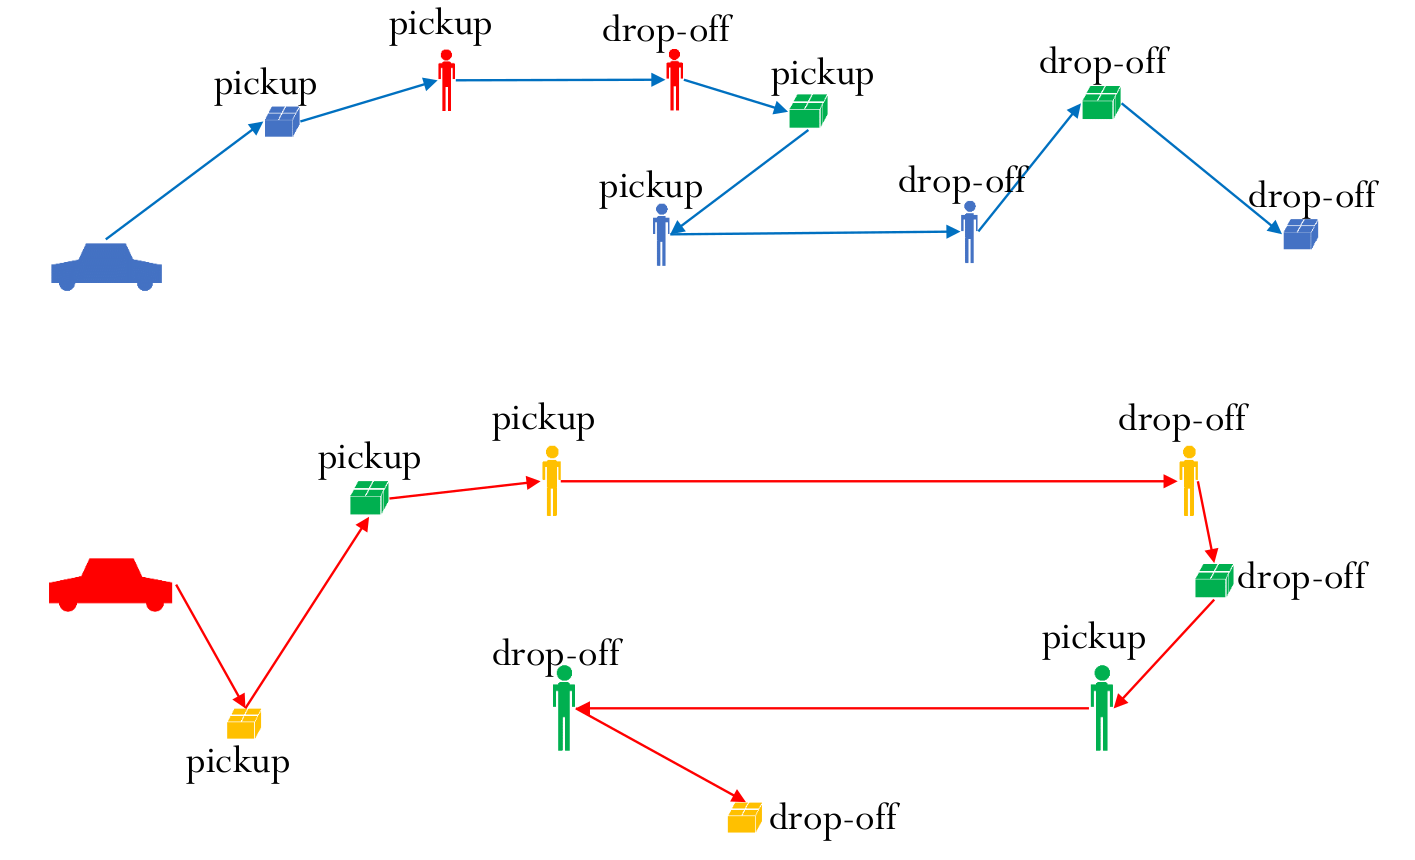
\includegraphics[width=0.8\textwidth]{../docs/taxi.png}
		\end{figure}
	\end{frame}
	
	%------------------------------------------------
	
%	\section{Các hướng tiếp cận}
%	
%	%------------------------------------------------
%	
%	\begin{frame}
%		\frametitle{Các hướng tiếp cận}
%		\begin{itemize}
%			\item Sử dụng các giải thuật chính xác
%			\item Sử dụng các giải thuật xấp xỉ
%		\end{itemize}
%	\end{frame}
%	
%	%------------------------------------------------
%	
%	\begin{frame}
%		\frametitle{Các hướng tiếp cận}
%		\begin{block}{Giải bài toán bằng thuật toán chính xác}
%			Lorem ipsum dolor sit amet, consectetur adipiscing elit. Integer lectus nisl, ultricies in feugiat rutrum, porttitor sit amet augue. Aliquam ut tortor mauris. Sed volutpat ante purus, quis accumsan dolor.
%		\end{block}
%	\end{frame}
%
%	%------------------------------------------------
%	
%	\begin{frame}
%		\frametitle{Các hướng tiếp cận}
%		\begin{block}{Giải bài toán bằng thuật toán xấp xỉ}
%			Lorem ipsum dolor sit amet, consectetur adipiscing elit. Integer lectus nisl, ultricies in feugiat rutrum, porttitor sit amet augue. Aliquam ut tortor mauris. Sed volutpat ante purus, quis accumsan dolor.
%		\end{block}
%	\end{frame}
	
	%------------------------------------------------
	
	\section{Mô hình bài toán}
	
	%------------------------------------------------
	
	\begin{frame}
		\frametitle{Mô hình bài toán}
		\textbf{\underline{Tham số}}
		\begin{itemize}
			\item Tập $2N+2M+2K$ điểm:
			\begin{itemize}
				\item Hành khách $i$: điểm đón $i$ và điểm trả $i+N+M$ ($i=1,2,...,N$)
				\item Gói hàng $j$: điểm lấy hàng $j$ và điểm trả $j+N+M$ ($j=N+1,N+2,...,N+M$)
				\item $2K$ điểm logic $2N+2M+1, 2N+2M+2, ..., 2N+2M+2K$ tham chiếu tới điểm xuất phát vật lý $0$. Điểm $2N+2M+k$ tương ứng là điểm bắt đầu, $2N+2M+K+k$ là điểm kết thúc lộ trình xe thứ $k$ ($k=1,2,...,K$)
			\end{itemize}
			\item $d_{ij}$: Khoảng cách từ điểm $i$ tới điểm $j$ ($i,j\in \{1,2,...,2N+2M+2K\}$)
			\item $w_i$: Sự thay đổi khối lượng hàng khi đi tới điểm $i$ ($i=1,2,...,2N+2M+2K$)
			\begin{equation}
				w_i =
				\begin{cases}
					q_i & \text{nếu } N+1\leq i\leq N+M\\
					-q_{i-(N+M)} & \text{nếu } 2N+M+1\leq i\leq 2N+2M\\
					0 & \text{ngược lại}
				\end{cases} \notag
			\end{equation}
			\item $Q_k$: Khối lượng hàng tối đa xe thứ $k$ có thể chở ($k=1,2,...,K$)
		\end{itemize}
	\end{frame}

	\begin{frame}
		\frametitle{Mô hình bài toán}
		\textbf{\underline{Biến quyết định}}
		\begin{itemize}
			\item $x_{ij}$: Biến nhị phân, xác định cung đi từ điểm $i$ đến điểm $j$ có xuất hiện trong lộ trình của 1 trong $k$ xe không ($i,j\in [1..(2N+2M+2K)]$)
			\begin{equation}
				x_{ij} = 
				\begin{cases}
				1 & \text{nếu cung $(i,j)$ có trong lộ trình của 1 xe}\\
				0 & \text{ngược lại}
				\end{cases}
			\end{equation}
			\item Tại mỗi điểm $i$ ($i\in [1..(2N+2M+2K)]$):
			\begin{itemize}
				\item $r_i$: chỉ số của xe đi qua điểm $i$ trong lộ trình
					\begin{equation}
					1\leq r_i\leq K
					\end{equation}
				\item $l_i$: khoảng cách tích lũy của xe đi từ điểm $0$ đến điểm $i$ trong lộ trình
					\begin{equation}
					0\leq l_i < \infty
					\end{equation}
				\item $c_i$: khối lượng hàng xe $k$ (đi qua điểm $i$) còn chịu được khi đi tới điểm $i$
					\begin{equation}
					0\leq c_i\leq \max _{1\leq k\leq K} \{Q_k\}
					\end{equation}
			\end{itemize}
		\end{itemize}
	\end{frame}

	\begin{frame}
		\frametitle{Mô hình bài toán}
		\textbf{\underline{Ràng buộc}} (ký hiệu $P=2N+2M$)
		\begin{itemize}
			\item Ràng buộc cân bằng luồng vào ra:
				\begin{align}
				\sum_{j=1}^{2N+2M+2K} x_{ij} = 1,\quad & \forall i\in [1..(P+K)] \\
				\sum_{i=1}^{2N+2M+2K} x_{ij} = 1,\quad & \forall j\in [1..P]\cup [(P+K+1)..(P+2K)]
				\end{align}
			\item Xác định $r_i$:
%			\begin{align}
%			f(x)=\begin{cases}
%			1, & i\in 1.\\
%			0, & \text{otherwise}.
%			\end{cases}
%			\end{align}
				\begin{equation}
					r_{2N+2M+k} = k,\quad \forall k=1,2,...,K
				\end{equation}
				\begin{align}
				\begin{cases}
				r_j - r_i\leq \mu\times (1 - x_{ij}), &\forall j\in [1...P]\cup [(P+K+1)...(P+2K)],\\ 
				r_j - r_i\geq -\mu\times (1 - x_{ij}) &i\in [1...(P+2K)], i\ne j
				\end{cases}
				\end{align}
		\end{itemize}
	\end{frame}

	\begin{frame}
		\frametitle{Mô hình bài toán}
		\begin{itemize}
			\item Xác định $l_i$:
				\begin{equation}
					l_{2N+2M+k} = 0,\quad k\in [1..K]
				\end{equation}
				\begin{align}
				\begin{cases}
				l_j - l_i -d_{ij}\leq \mu\times (1 - x_{ij}), & \forall j\in [1..P]\cup [(P+K+1)..(P+2K)], \\
				l_j - l_i -d_{ij}\geq -\mu\times (1 - x_{ij}) & i\in [1..(P+2K)], i\ne j
				\end{cases}
				\end{align}
			\item Xác định $c_i$:
				\begin{equation}
				c_{2N+2M+k} = Q_k,\quad k\in [1..K]
				\end{equation}
				\begin{align}
				\begin{cases}
				c_j - c_i - w_j\leq \mu\times (1 - x_{ij}), & \forall j\in [1..P]\cup [(P+K+1)..(P+2K)], \\
				c_j - c_i - w_j\geq -\mu\times (1 - x_{ij}) & i\in [1..(P+2K)], i\ne j
				\end{cases}
				\end{align}
		\end{itemize}
	\end{frame}

	\begin{frame}
		\frametitle{Mô hình bài toán}
		\begin{itemize}
			\item Điểm đón và trả của hành khách $i$ phải thuộc lộ trình của cùng một xe, tương tự với các gói hàng:
				\begin{align}
				r_i = r_{i+N+M},\quad & \forall i\in [1..(N+M)]
				\end{align}
			\item Điểm đón khách phải liền trước điểm trả khách:
				\begin{align}
				x_{i,(i+N+M)} = 1,\quad & \forall i\in [1..N]
				\end{align}
			\item Điểm lấy hàng phải ở trước điểm giao hàng:
				\begin{align}
				l_i \leq l_{i+N+M},\quad & \forall i\in [(N+1)..(N+M)]
				\end{align}
			\item Khối lượng còn lại của xe tại mọi thời điểm không âm (đã thỏa mãn).
		\end{itemize}
	\end{frame}

	\begin{frame}
		\frametitle{Mô hình bài toán}
		\begin{itemize}
			\item $L$: Độ dài của lộ trình xe dài nhất trong $K$ lộ trình
			\item Ràng buộc xác định lộ trình dài nhất:
				\begin{align}
				l_i\leq L,\quad & \forall i\in [(P+K+1)..(P+2K)]
				\end{align}
		\end{itemize}
		\textbf{\underline{Hàm mục tiêu}}
			\begin{equation}
			L \leftarrow min
			\end{equation}
	\end{frame}

	%------------------------------------------------
	
	\section{Giải thuật chính xác}
	
	%------------------------------------------------
	
	\subsection{Mô hình MIP}
	\begin{frame}
		\frametitle{Mô hình MIP}
		\begin{itemize}
			\item Mô hình MIP đã trình bày ở trên.
			\item Sử dụng thư viện OR-Tools (Java) để triển khai.
		\end{itemize}
	\end{frame}

	\subsection{Thuật toán nhánh cận}
	\begin{frame}
		\frametitle{Thuật toán nhánh cận}
		\textbf{Phương pháp:}
		\begin{itemize}
			\item \underline{Khởi tạo:} Lời giải rỗng, lộ trình mỗi xe chỉ có điểm đầu $0$ và điểm cuối $0$.
			\item \underline{Trạng thái nút:} Đang xét xe thứ $k$, đã xây xong lộ trình các xe trước.
			\item {
				\underline{Rẽ nhánh:} Thực hiện một trong các thao tác:
				\begin{itemize}
					\item Chọn 1 khách chưa được phục vụ, thêm liên tiếp điểm đón và điểm trả khách vào cuối lộ trình xe $k$
					\item Chọn 1 gói hàng chưa có xe lấy, thêm điểm lấy hàng vào cuối lộ trình
					\item Chọn 1 gói hàng mà xe $k$ đã lấy nhưng chưa giao, thêm điểm giao hàng vào cuối lộ trình
					\item Kết thúc xây lộ trình xe $k$, chuyển sang xe $k+1$
				\end{itemize}
			}
			\item \underline{Tỉa nhánh:} Các nút có lộ trình xe $k$ dài hơn lời giải tốt nhất hiện tại.
		\end{itemize}
	\end{frame}
	
	%------------------------------------------------
	
	\section{Giải thuật heuristics}
	
	%------------------------------------------------
	
	\subsection{Giải thuật di truyền}
	
	\begin{frame}
		\frametitle{Giải thuật di truyền}
		\begin{itemize}
			\item Sử dụng giải thuật di truyền cho các bộ dữ liệu kích thước lớn
			\item Tìm ra lời giải tối ưu cục bộ
		\end{itemize}
		\begin{figure}
			\centering
			\caption{Sơ đồ giải thuật di truyền}
			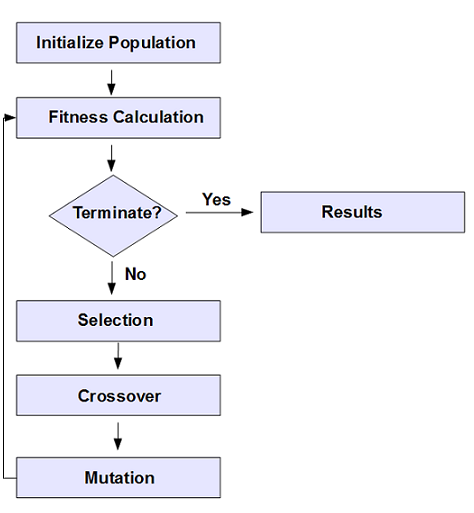
\includegraphics[width=0.4\textwidth]{images/ga-flow.png}
		\end{figure}
	\end{frame}

	\begin{frame}
		\frametitle{Giải thuật di truyền}
		\textbf{Toán tử lai ghép:} Phép lai ghép làm đổi lại thứ tự của các hành khách trong hành trình
		\begin{itemize}
			\item Chọn ra tập cha mẹ bằng phương pháp tournament
			\item Đối với từng cặp lời giải, xác suất xảy ra lai ghép là $P_c$
			\item Xét cặp lời giải bất kì trong tập cha mẹ gồm lời giải $S_p$ và $S_q$:
				\begin{itemize}
					\item Gọi cặp hành trình $r_i$ và $r_j$ ($r_i \in S_p$ và $r_j \in S_q$) là cặp hành trình tương đồng nếu có số hành khách trùng nhau là lớn nhất
					\item Sắp xếp lại thứ tự đón các hành khách chung của $r_i$ và $r_j$ trong $r_i$ theo $r_j$ ta được lời giải mới
				\end{itemize}
		\end{itemize}
	
		\textbf{Toán tử đột biến:}
		\begin{itemize}
			\item Di chuyển một món hàng hóa từ route có độ dài lớn nhất sang route có độ dài nhỏ nhất
			\item Di chuyển Hoán đổi khách hàng giữa 2 route bất kì
		\end{itemize}
	\end{frame}
	
	\subsection{Thuật toán tham lam}
	\begin{frame}
		\frametitle{Thuật toán tham lam}
		\textbf{Các bước thực hiện:}
		\begin{itemize}
			\item \underline{Bước 0:} Khởi tạo lời giải rỗng.
			\item {
				\underline{Bước 1:} Thêm các yêu cầu chuyển hàng:
				\begin{itemize}
					\item Duyệt qua các gói hàng chưa xử lý.
					\item Duyệt tất cả các cặp vị trí (thuộc cùng 1 xe) có thể chèn điểm lấy và điểm giao hàng (mà không vi phạm ràng buộc).
					\item Chọn một trong các cặp vị trí làm lộ trình được chèn có độ dài mới là nhỏ nhất.
				\end{itemize}
			}
			\item {
				\underline{Bước 2:} Thêm các yêu cầu chuyển người:
				\begin{itemize}
					\item Duyệt qua các yêu cầu chờ khách chưa xử lý.
					\item Duyệt tất cả các vị trí để chèn cặp điểm đón và điểm trả người (mà không vi phạm ràng buộc).
					\item Chọn một trong các vị trí làm lộ trình được chèn có độ dài mới là nhỏ nhất.
				\end{itemize}
			}
		\end{itemize}
		\textbf{Độ phức tạp:} $O(\max \{ M\times (2M+2N+K)^3, N\times (2M+2N+K)^2 \})$
	\end{frame}

	\renewcommand\AlCapFnt{\scriptsize}
	\renewcommand\AlCapNameFnt{\scriptsize}
	\begin{frame}
		\frametitle{Thuật toán tham lam}
		\begin{algorithm}[H]
			\fontsize{7pt}{7pt}\selectfont
			
			\KwIn{
				$S$: The station of $K$ taxis; \\
				$Taxis$: List of $K$ taxis; \\
				$People$: List of $N$ passenger transport requests; \\
				$Goods$: List of $M$ commodity delivery requests;
			}
			\KwOut{$K$ routes which balance the traveling distances of $K$ taxis}
			
			\BlankLine
			$mgr\leftarrow$ Vehicle routing manager for $K$ taxis\;
			  
			\ForEach{$g \in Goods$} {
				$(x_1,x_2)\leftarrow$ pickup and delivery points of $g$\;
				
				\ForEach{Route $r_k \in mgr$} {
					\ForEach{Pair $(y_1,y_2) \in r_k$}{
						$mgr\rightarrow$ evaluate inserting $x_1$ behind $y_1$, $x_2$ behind $y_2$\;
						$\Rightarrow l_{y_1y_2}$: The new length of route $r_k$\;
					}
				}
				Find pair $(y_1,y_2)$ with no violation and $l_{y_1y_2}\leftarrow min$\;
				$mgr\rightarrow$ insert $x_1$ behind $y_1$, $x_2$ behind $y_2$\;
			}
		
			\ForEach{$p \in People$} {
				$(x_1,x_2)\leftarrow$ pickup and delivery points of $p$\;
				
				\ForEach{Route $r_k \in mgr$} {
					\ForEach{$y \in r_k$}{
						$mgr\rightarrow$ evaluate inserting $(x_1,x_2)$ behind $y$\;
						$\Rightarrow l_y$: The new length of route $r_k$\;
					}
				}
				Find point $y$ with no violation and $l_y\leftarrow min$\;
				$mgr\rightarrow$ insert $(x_1,x_2)$ behind $y$\;
			}
		
			\caption{Greedy algorithm}
		\end{algorithm}
	\end{frame}
	
	%------------------------------------------------
	
	\subsection{Tìm kiếm cục bộ}
	\begin{frame}
		\frametitle{Tìm kiếm cục bộ}
		\textbf{Các bước thực hiện:}
		\begin{itemize}
			\item \underline{Khởi tạo:} Sử dụng thuật toán tham lam đã trình bày.
			\item {
				\underline{Quá trình tìm kiếm:}
				\begin{itemize}
					\item Tìm một lời giải hàng xóm tốt hơn lời giải hiện tại.
					\item Nếu không, tìm lời giải tốt nhất trong các hàng xóm, tạm thay lời giải hiện tại.
					\item Nếu đã qua một số vòng lặp mà lời giải hiện tại không cải thiện, khởi tạo lại lời giải.
					\item Cập nhật lời giải tốt nhất (nếu có thể).
				\end{itemize}
			}
			\item Lặp lại quá trình trên tới khi chạm số vòng lặp hoặc thời gian chạy tối đa.
		\end{itemize}
	\end{frame}

	\begin{frame}
		\frametitle{Tìm kiếm cục bộ}
		\textbf{Xây dựng tập lời giải hàng xóm:}
		\begin{itemize}
			\item {\underline{Move 1:} Dịch vị trí điểm lấy và giao hàng:
				\begin{itemize}
					\item $x_1,x_2$ là điểm lấy và giao cùng một gói hàng
					\item Chọn 2 điểm $y_1, y_2$ thuộc cùng lộ trình
					\item Bỏ $x_1, x_2$ khỏi lộ trình hiện tại, chèn $x_1$ sau $y_1$, $x_2$ sau $y_2$
				\end{itemize}
			}
			\item {\underline{Move 2:} Dịch vị trí cặp điểm đón trả khách:
				\begin{itemize}
					\item $x_1,x_2$ là điểm đón và trả cùng một gói hàng
					\item Chọn điểm $y$ bất kỳ trong các lộ trình
					\item Bỏ $x_1, x_2$ khỏi lộ trình hiện tại, chèn $x_1,x_2$ liên tiếp sau $y$
				\end{itemize}
			}
		\end{itemize}
		
	\end{frame}

	\begin{frame}
		\frametitle{Tìm kiếm cục bộ}
		\begin{figure}
			\centering
			\caption{Move 1: Dịch vị trí gói hàng}
			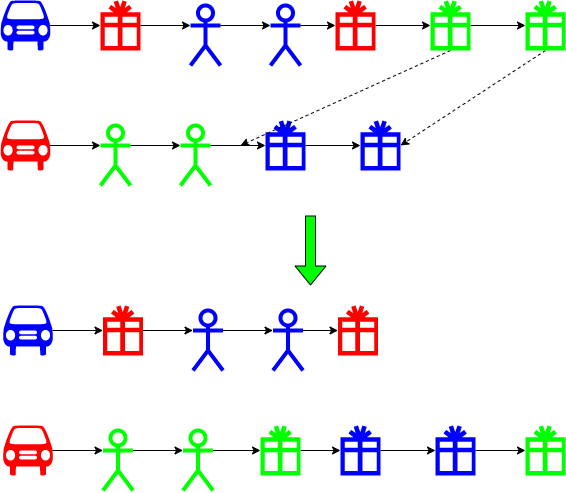
\includegraphics[width=0.6\textwidth]{images/cbls-good.png}
		\end{figure}
	\end{frame}

	\begin{frame}
		\frametitle{Tìm kiếm cục bộ}
		\begin{figure}
			\centering
			\caption{Move 2: Dịch vị trí hành khách}
			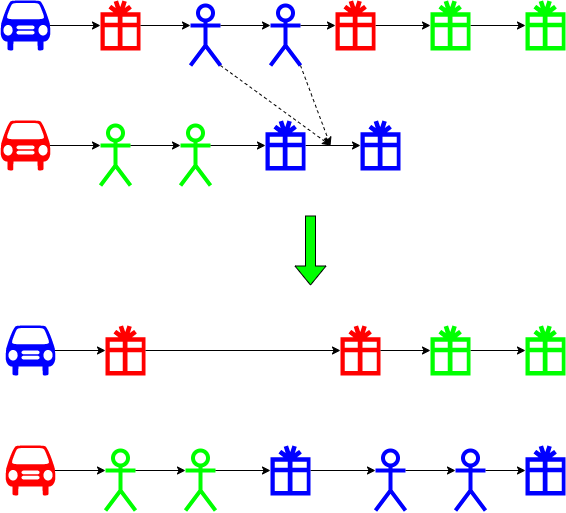
\includegraphics[width=0.6\textwidth]{images/cbls-people.png}
		\end{figure}
	\end{frame}
	
	%------------------------------------------------
	\section{Thực nghiệm}
	



	%------------------------------------------------
	
	\subsection{Tham số thuật toán}
	\begin{frame}
	\frametitle{Tham số thuật toán}
		\begin{itemize}
			\item Số lần chạy heuristics / bộ dữ liệu: 10
			\item {
				Tìm kiếm cục bộ:
				\begin{itemize}
					\item Số vòng lặp: 100
					\item Số bước cho phép lời giải tồi: 10
					\item Giới hạn thời gian: 5 phút
				\end{itemize}
			}
			\item {
				Giải thuật di truyền:
				\begin{itemize}
					\item Kích thước quần thế khởi tạo: 200
					\item Số thế hệ: 500
					\item Xác suất lai ghép: 0.5
					\item Xác suất đột biến: 0.1
				\end{itemize}
			}
		\end{itemize}
	\end{frame}

	\subsection{Kết quả thực nghiệm}
	\begin{frame}
		\frametitle{Kết quả thực nghiệm}
		\begin{figure}
			\centering
			\caption{Thực nghiệm giải thuật chính xác}
			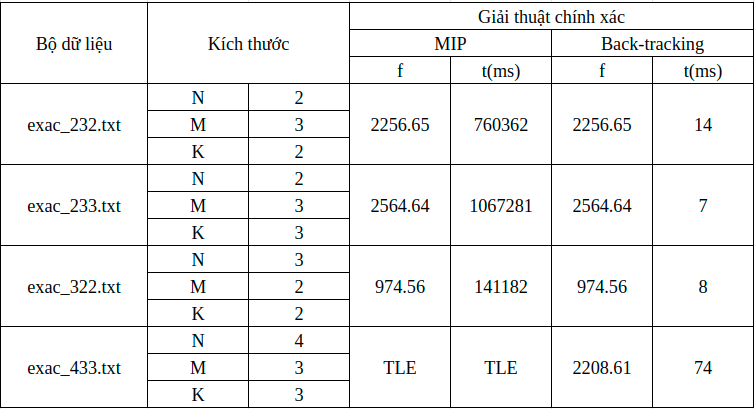
\includegraphics[width=0.8\textwidth]{images/exac.png}
		\end{figure}
	\end{frame}

	\begin{frame}
		\frametitle{Kết quả thực nghiệm}
		\begin{figure}
			\centering
			\caption{Minh họa kết quả giải thuật chính xác}
			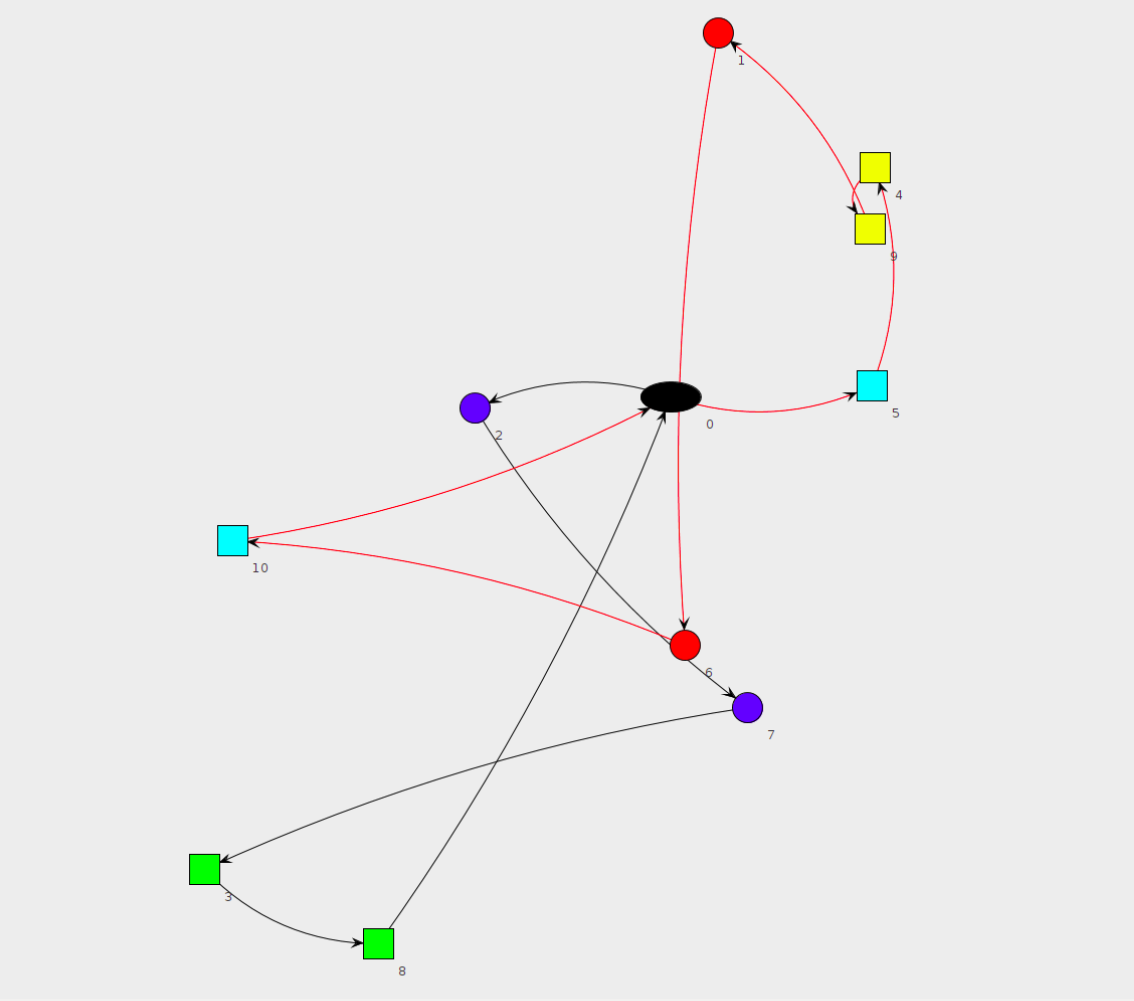
\includegraphics[width=0.6\textwidth]{../result/image/solution.png}
		\end{figure}
	\end{frame}

	\begin{frame}
		\frametitle{Kết quả thực nghiệm}
		\begin{figure}
			\centering
			\caption{Thực nghiệm giảt thuật di truyền}
			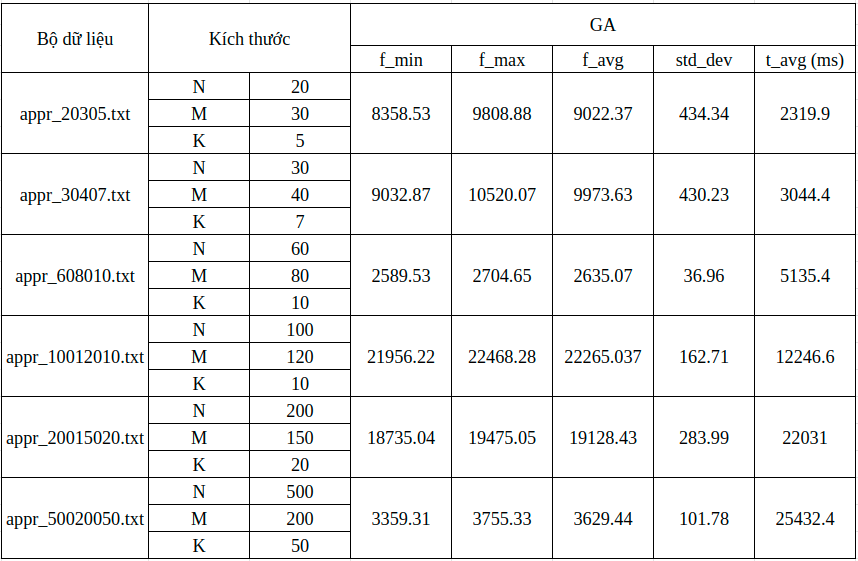
\includegraphics[width=0.8\textwidth]{images/ga.png}
		\end{figure}
	\end{frame}

	\begin{frame}
		\frametitle{Kết quả thực nghiệm}
		\begin{figure}
			\centering
			\caption{Thực nghiệm giải thuật tham lam}
			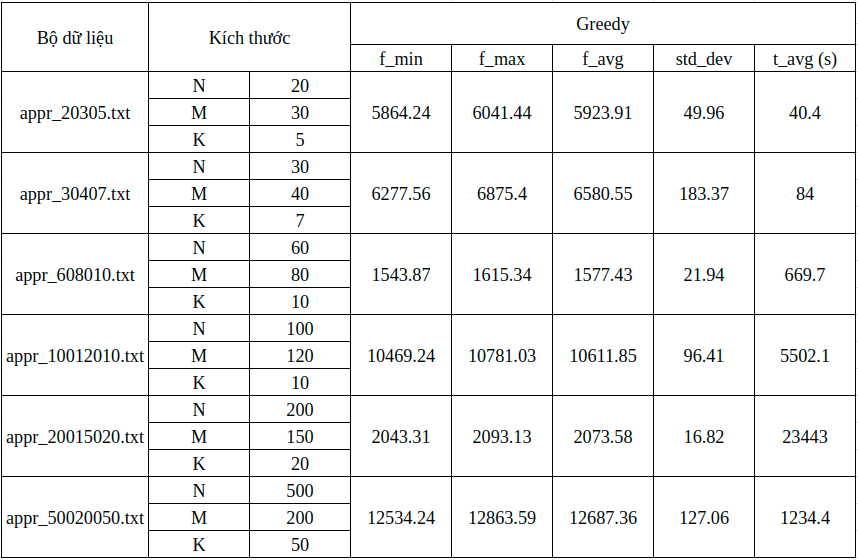
\includegraphics[width=0.8\textwidth]{images/greedy.png}
		\end{figure}
	\end{frame}

	\begin{frame}
		\frametitle{Kết quả thực nghiệm}
		\begin{figure}
			\centering
			\caption{Thực nghiệm giải thuật tìm kiếm cục bộ}
			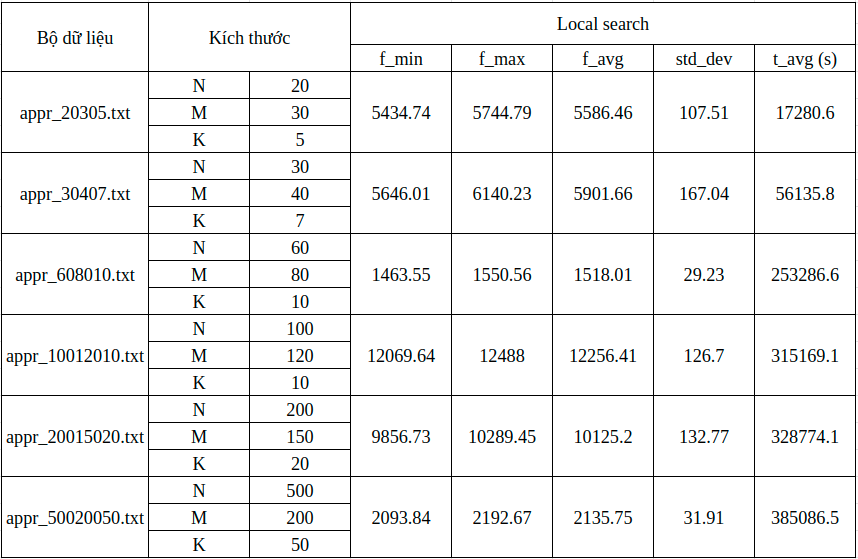
\includegraphics[width=0.8\textwidth]{images/localsearch.png}
		\end{figure}
	\end{frame}

	\begin{frame}
		\frametitle{Kết quả thực nghiệm}
		\begin{figure}
			\centering
			\caption{So sánh các giải thuật xấp xỉ}
			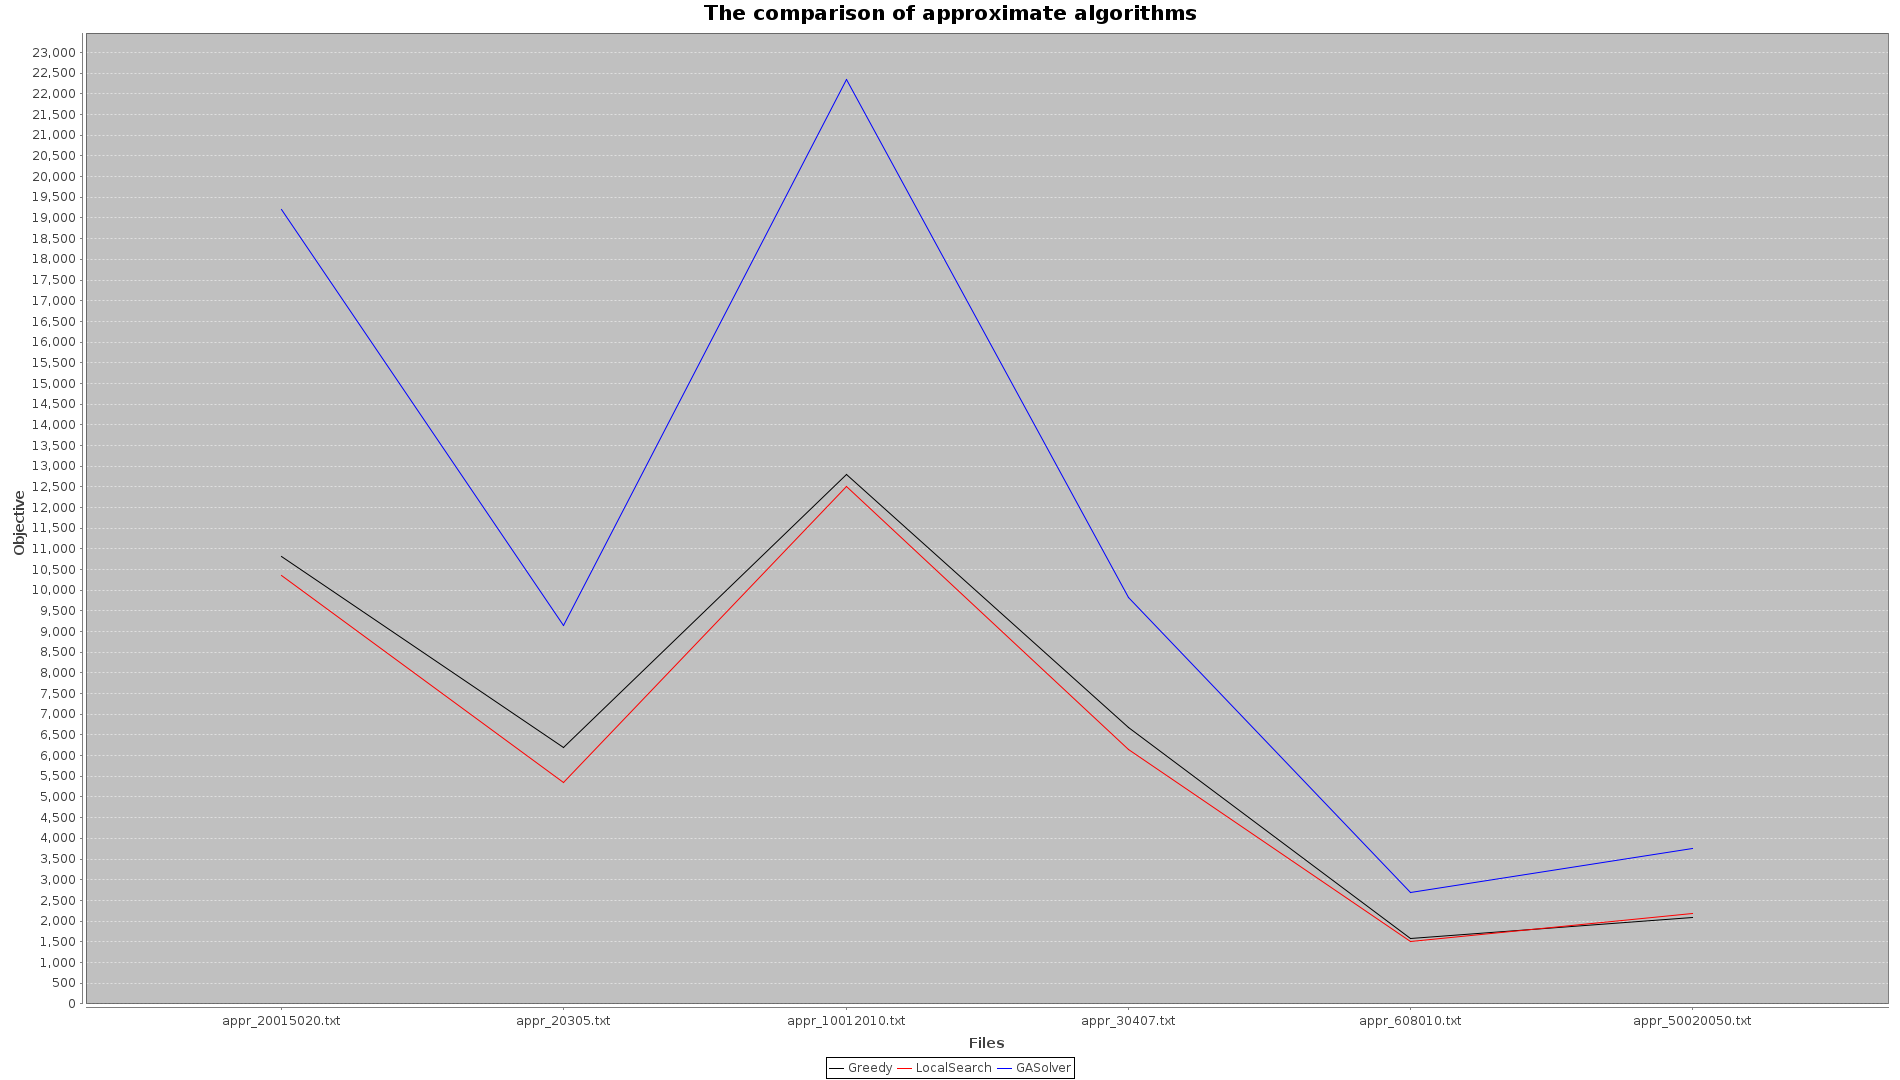
\includegraphics[width=\textwidth]{../result/image/comparison.png}
		\end{figure}
	\end{frame}
	\begin{frame}
		\frametitle{Kết quả thực nghiệm}
		\begin{figure}
			\centering
			\caption{So sánh tất cả giải thuật trên bộ exac}
			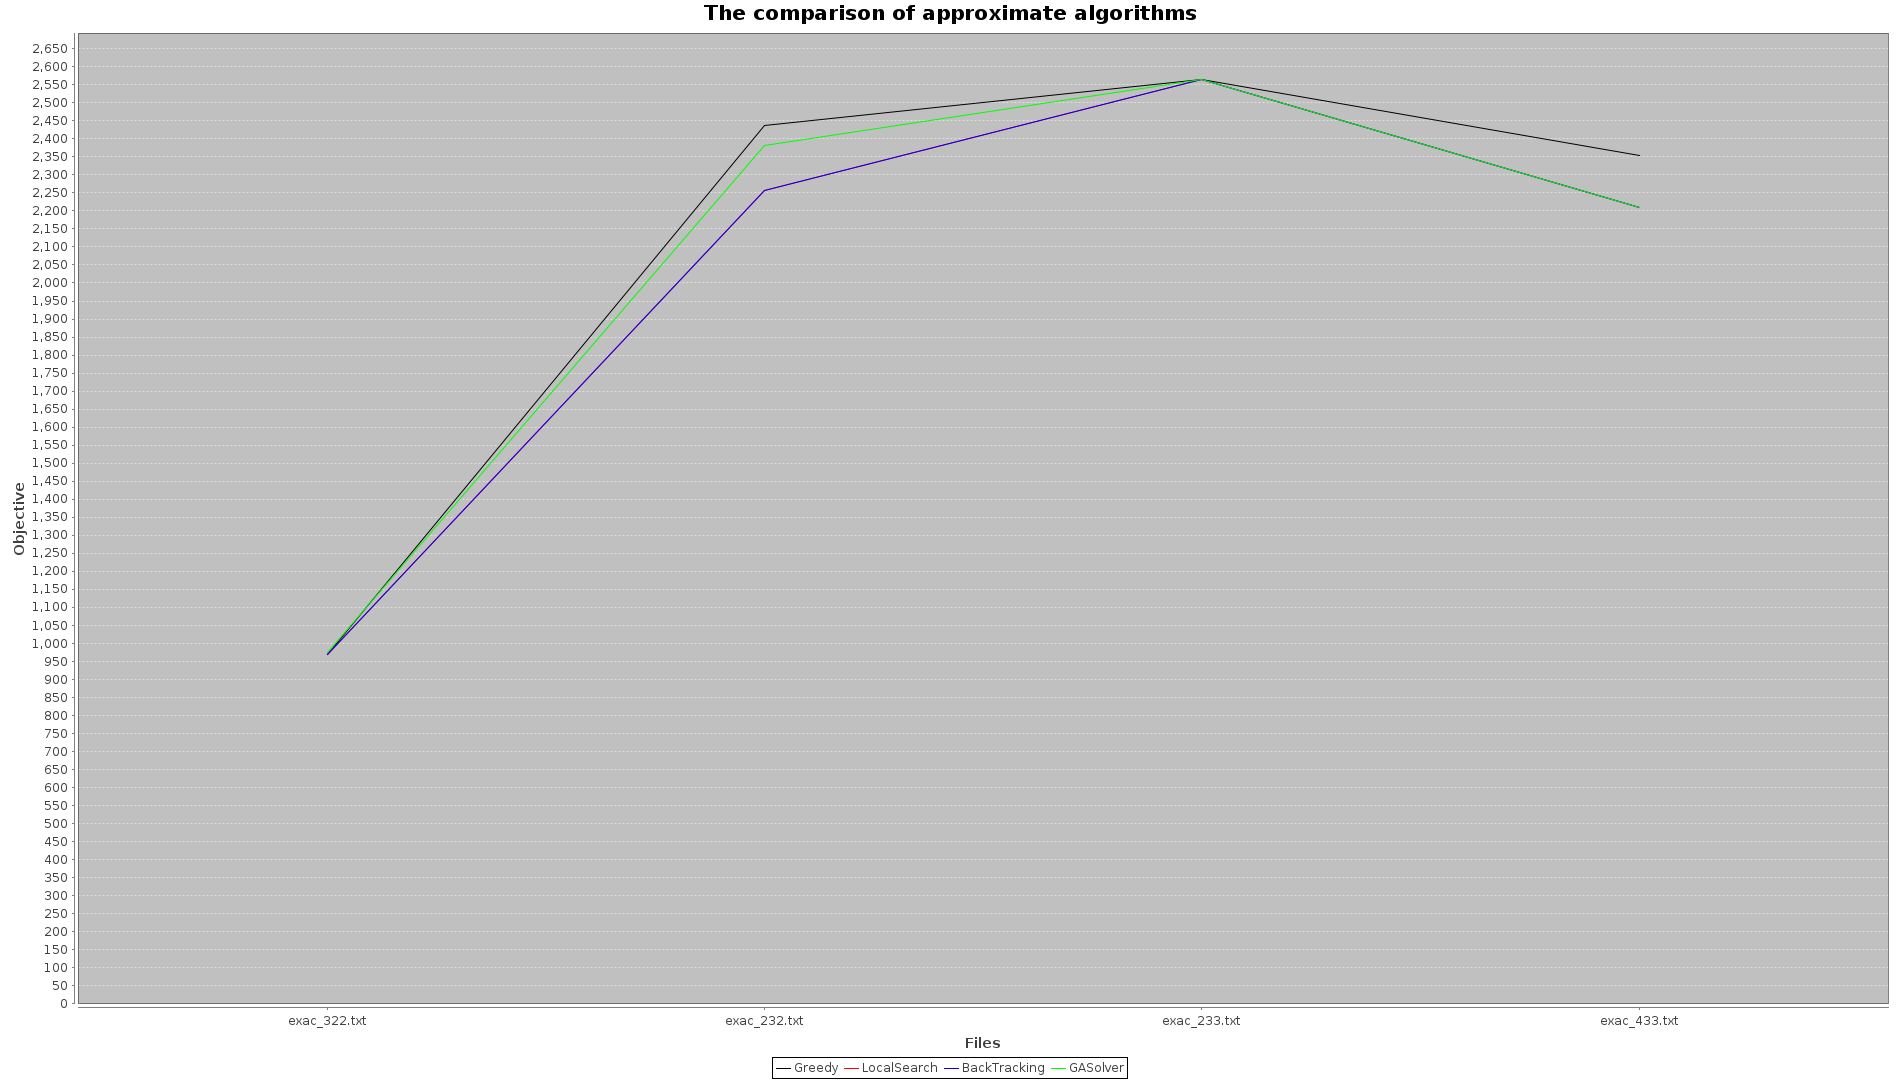
\includegraphics[width=\textwidth]{../result/image/comp.png}
		\end{figure}
	\end{frame}

	%------------------------------------------------
	
	\section{Kết luận và phân công công việc}
	
	%------------------------------------------------
	
	\begin{frame}
		\frametitle{Kết luận}
		\begin{itemize}
			\item Mô hình MIP đã đề xuất cho kết quả chính xác, tuy nhiên thời gian chạy lớn hơn rất nhiều so với giải thuật nhánh cận.
			\item Đối với các bộ dữ liệu kích thước lớn, thuật toán tìm kiếm cục bộ cho hiệu quả tốt nhất
		\end{itemize}
	\end{frame}

	\begin{frame}
		\frametitle{Phân công công việc}
		\begin{itemize}
			\item {Trần Huy Hùng - 20164777
				\begin{itemize}
					\item Mô hình MIP
					\item {Triển khai:
						\begin{itemize}
							\item Thuật toán nhánh cận
							\item Thuật toán tham lam
							\item Tìm kiếm cục bộ
						\end{itemize}
					}
					\item Slide
				\end{itemize}
			}
			\item {Đỗ Ngọc Sơn - 20163506
				\begin{itemize}
					\item Mô hình MIP
					\item {Triển khai:
						\begin{itemize}
							\item Giải thuật di truyền
						\end{itemize}
					}
					\item {Thực nghiệm:
						\begin{itemize}
							\item Sinh dữ liệu
							\item Thống kê và visualize kết quả
						\end{itemize}
					}
					\item Slide
				\end{itemize}
			}
		\end{itemize}
	\end{frame}
	
\end{document} 